\documentclass[11pt,a4paper]{ctexart}

\usepackage[margin=2.6cm]{geometry}
\usepackage{amsmath,amssymb,amsthm}
\usepackage{graphicx}
\usepackage{booktabs}
\usepackage{hyperref}
\usepackage{xcolor}
\usepackage{listings}
\usepackage{caption}

\graphicspath{{figures/}}
\hypersetup{colorlinks=true, linkcolor=blue!50!black, urlcolor=blue!60!black}
\lstset{
  basicstyle=\ttfamily\small,
  breaklines=true,
  frame=single,
  columns=fullflexible,
  backgroundcolor=\color{gray!7}
}

\newtheorem{definition}{定义}[section]
\newtheorem{theorem}{定理}[section]
\newtheorem{lemma}{引理}[section]
\newtheorem{proposition}{命题}[section]
\newtheorem{example}{例}[section]

\title{第 12 章 \quad Multivariate time series / 多元时间序列}
\author{基于 \textit{A Course in Time Series Analysis} 的中文讲义与 Python 实践}
\date{}

\begin{document}
\maketitle

\section*{本章学习目标}

本章按照原文 \textit{Multivariate time series} 的小节顺序整理，保留主要定义、定理、模型公式和练习方向，并将原文中的 R 实践思路改写为 Python 工程实践。

完成本章后，应能够：
\begin{itemize}
  \item 复习序列卷积和矩阵谱表示；
  \item 建立多元时间序列回归模型；
  \item 理解条件独立、偏相关和相干性；
  \item 定义交叉谱密度和谱偏相关；
  \item 解释逆谱密度矩阵的条件依赖含义。
\end{itemize}

\section{背景}

\subsection{序列与卷积}

若 \(a=\{a_j\}\)、\(b=\{b_j\}\)，卷积定义为
\[
  (a*b)_k=\sum_j a_jb_{k-j}.
\]
多元线性滤波中，系数可为矩阵，卷积描述不同序列和不同滞后之间的相互作用。

\subsection{谱表示}

多元平稳序列 \(X_t\in\mathbb R^d\) 的自协方差矩阵为
\[
  \Gamma(h)=E(X_{t+h}X_t').
\]
谱密度矩阵定义为
\[
  f(\omega)=\frac1{2\pi}\sum_{h=-\infty}^{\infty}\Gamma(h)e^{-ih\omega}.
\]
它在每个频率上是 Hermitian 非负定矩阵。

\section{多元时间序列回归}

多元线性模型可写为
\[
  Y_t=\sum_{j}A_jX_{t-j}+\varepsilon_t.
\]
向量自回归 VAR(p) 是典型例子：
\[
  X_t=A_1X_{t-1}+\cdots+A_pX_{t-p}+\varepsilon_t.
\]
矩阵 \(A_j\) 描述一个变量过去值对另一个变量当前值的动态影响。

\subsection{条件独立}

若一个分量在给定其他序列后不能由另一分量改善预测，则称二者条件线性不相关。高斯情形下，这可进一步解释为条件独立。

\section{偏相关、相干性与交叉谱}

两个序列的交叉谱密度 \(f_{12}(\omega)\) 是交叉协方差的 Fourier 变换。相干性定义为
\[
  \mathrm{coh}_{12}(\omega)
  =\frac{|f_{12}(\omega)|^2}{f_{11}(\omega)f_{22}(\omega)}.
\]
它是频域中的相关系数平方，取值在 \([0,1]\)。

谱偏相关是在给定其他序列后定义的频域相关，类似多元分析中的偏相关。

\section{逆谱密度矩阵}

设
\[
  g(\omega)=f(\omega)^{-1}.
\]
逆谱密度矩阵的零元素表示频域条件不相关结构。对高斯平稳序列，若 \(g_{ij}(\omega)=0\) 对所有 \(\omega\) 成立，则第 \(i\) 和第 \(j\) 个序列在给定其他序列后条件独立。

原文还证明了公式 (12.6)，把谱偏相关和逆谱密度矩阵联系起来。这一结构是高维多元时间序列图模型的基础。

\section{Python 工程实践}

在本章目录下运行：
\begin{lstlisting}[language=bash]
python scripts/ch12_generate_figures.py
\end{lstlisting}

脚本会把图像写入本章 \texttt{figures/} 目录。当前图像用于配合本章核心概念的仿真说明；若后续补齐原始数据文件，可把模拟数据替换为原文真实数据案例。

\begin{figure}[htbp]
  \centering
  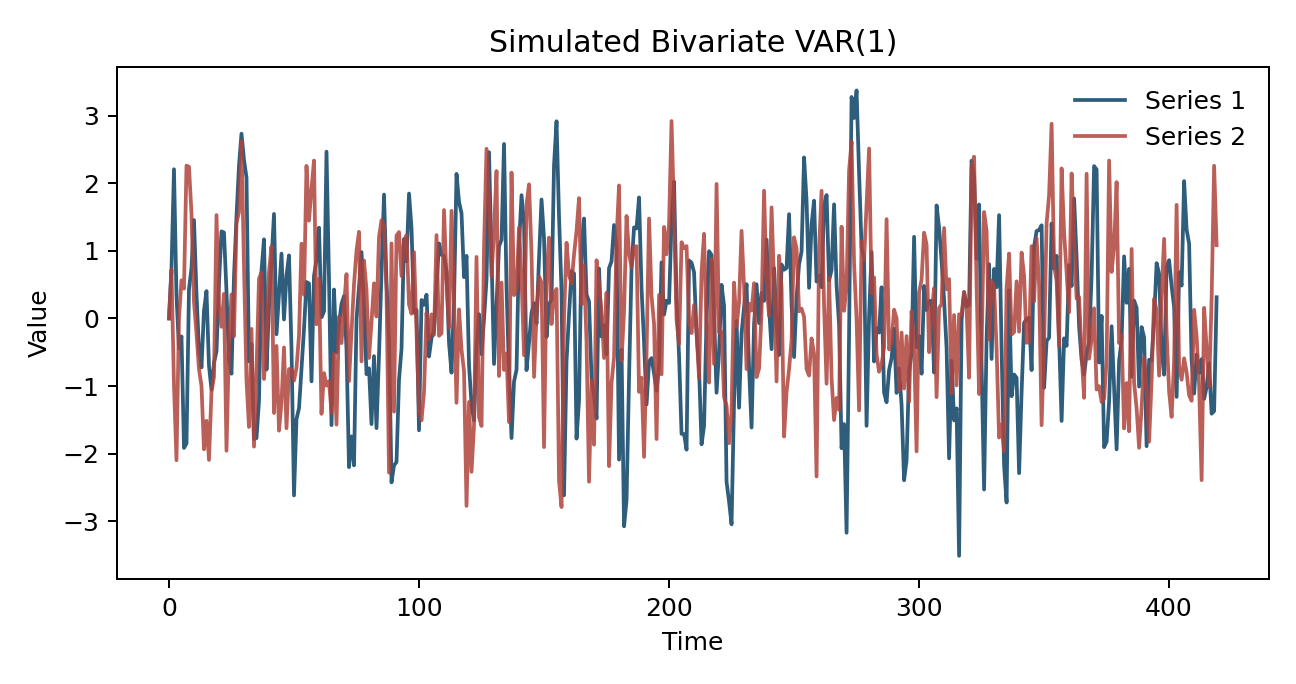
\includegraphics[width=0.86\textwidth]{ch12_fig01_var_series.png}
  \caption{二元 VAR(1) 模拟序列：两个变量通过滞后矩阵相互影响。}
\end{figure}

\begin{figure}[htbp]
  \centering
  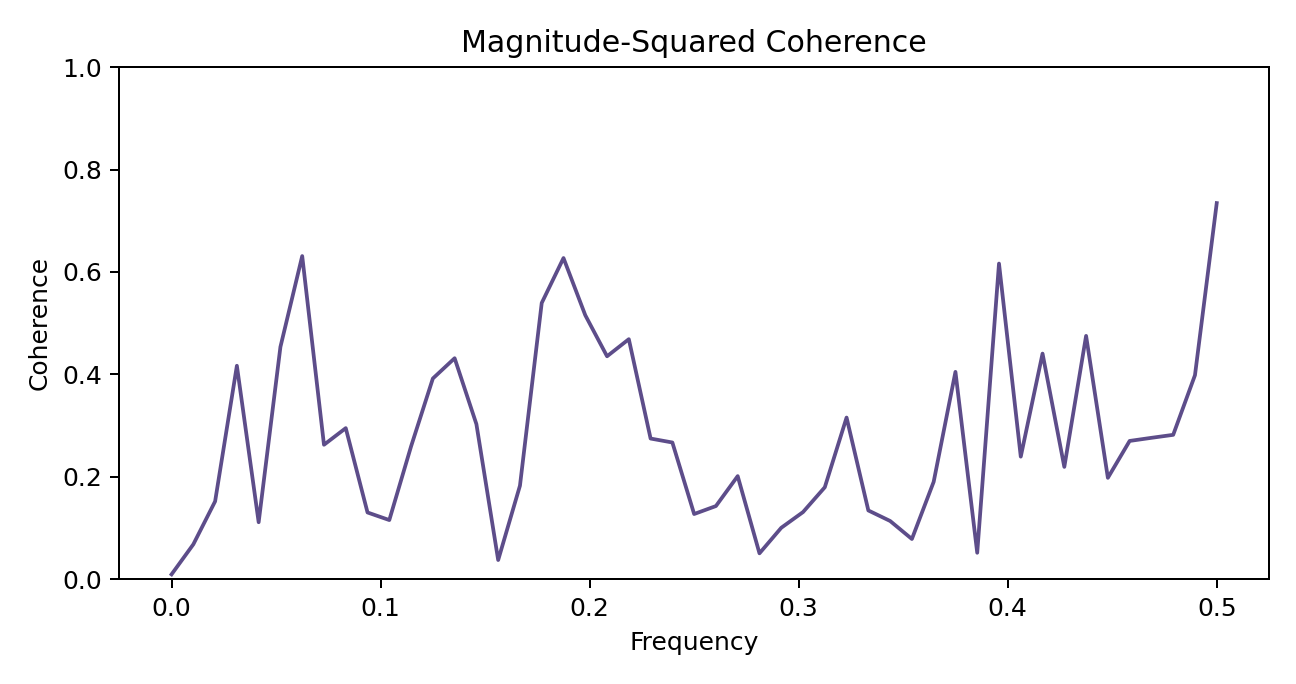
\includegraphics[width=0.86\textwidth]{ch12_fig02_coherence.png}
  \caption{相干性曲线：展示两个序列在不同频率上的线性关联强度。}
\end{figure}

\section{练习提要}

原文练习主要围绕下列方向展开：
\begin{itemize}
  \item 计算二元 VAR 的自协方差矩阵；
  \item 估计交叉谱和相干性；
  \item 解释逆谱密度矩阵零元素；
  \item 比较时域偏相关与频域谱偏相关。
\end{itemize}

\section*{本章小结}

第 12 章把单变量频域理论推广到矩阵情形。多元序列的关键不只是每个变量自身的谱密度，还包括交叉谱、相干性和逆谱密度所揭示的条件依赖网络。

\end{document}
